\documentclass[11pt]{article}

% ----- preamble -----
\usepackage[a4paper,margin=1.8cm]{geometry}
\usepackage{amsmath,amssymb}
\usepackage{alltt}
\usepackage{tikz}
\usepackage{tikz-cd}
\usetikzlibrary{arrows.meta,positioning,calc,fit,backgrounds,
  shapes.geometric,chains,decorations.pathreplacing}
\usepackage[most]{tcolorbox}
\usepackage{parskip}
\usepackage{xcolor}

\definecolor{ink}{RGB}{40,40,40}
\definecolor{soft}{RGB}{245,245,248}
\definecolor{grn}{RGB}{30,140,80}

% the two brick colours + one connective + assembly
\definecolor{faceF}{RGB}{200,140,0}   % Frobenius / doubling   F
\definecolor{faceL}{RGB}{30,140,80}   % linearized loop        L
\definecolor{conn}{RGB}{30,110,190}   % telescope connective
\definecolor{asm}{RGB}{150,60,160}    % assembly / paper objects
\definecolor{res}{RGB}{190,50,60}     % headline result

\newtcolorbox{note}[1][]{colback=soft,colframe=ink,boxrule=0.4pt,
  arc=2pt,left=6pt,right=6pt,top=4pt,bottom=4pt,#1}
\newtcolorbox{leanbox}[1][]{colback=black!4,colframe=black!55,boxrule=0.4pt,
  arc=1.5pt,left=5pt,right=5pt,top=3pt,bottom=3pt,#1}

% code block: alltt keeps ^ _ % $ literal, but \( \) { } still give math/groups
\newenvironment{lean}{\begin{leanbox}\begin{alltt}\small}{\end{alltt}\end{leanbox}}

\tikzset{
  obj/.style={draw=ink,rounded corners=3pt,fill=soft,inner sep=5pt,font=\small,align=center},
  brick/.style={draw=ink,rounded corners=2pt,inner sep=6pt,font=\small,align=center,
    minimum height=13mm},
  thm/.style={draw=ink,rounded corners=3pt,fill=white,inner sep=4pt,
    font=\small,align=center,minimum height=9mm},
  arr/.style={-{Stealth[length=2.5mm]},thick},
  dep/.style={-{Stealth[length=2.4mm]},thick,ink},
  badge/.style={circle,inner sep=0pt,minimum size=3.8mm,font=\scriptsize\bfseries,text=white},
}
\newcommand{\bF}{{\colorbox{faceF}{\textcolor{white}{\scriptsize\bfseries F}}}}
\newcommand{\bL}{{\colorbox{faceL}{\textcolor{white}{\scriptsize\bfseries L}}}}
\newcommand{\bT}{{\colorbox{conn}{\textcolor{white}{\scriptsize\bfseries T}}}}
\newcommand{\ck}{\textcolor{grn}{\checkmark}}
\newcommand{\lc}[1]{\texttt{\small #1}}

\title{\vspace{-1.5cm}\textbf{The \texttt{DobbertinLego} library}\\[4pt]
\large Two bricks \bF\ \bL, one connective \bT\ $\to$ Dobbertin's Theorem~1, step
$(1)\Rightarrow(2)$}
\author{\small A picture book of the minimal \texttt{DobbertinLego} Lean library
--- \texttt{import DobbertinLego}}
\date{}

\begin{document}
\maketitle
\vspace{-1.0cm}

\begin{note}
\textbf{What this is.} A deliberately minimal, end-to-end rebuild of the first
step of the proof of Theorem~1 in Dobbertin's 1999 paper \emph{Kasami Power
Functions, Permutation Polynomials and Cyclic Difference Sets} --- the
implication equation~(1)\,$\Rightarrow$\,equation~(2). The point of this version
is that the \emph{entire} proof snaps together from just \textbf{two primitive
bricks} and \textbf{one connective}:
\begin{center}
\bF\ Frobenius \lc{frob}\qquad
\bL\ linearized loop \lc{loop}\qquad
\bT\ telescope \lc{loop\_telescope}.
\end{center}
Every box drawn below is a \ck\ \lc{sorry}-free Lean declaration; the headline
depends only on the standard axioms \lc{propext}, \lc{Classical.choice},
\lc{Quot.sound}. The four modules are \lc{DobbertinLego/Frobenius},
\lc{DobbertinLego/Loop}, \lc{DobbertinLego/Assembly} and the root
\lc{DobbertinLego}.
\end{note}

%=====================================================================
\section*{The whole library on one page}

\begin{center}
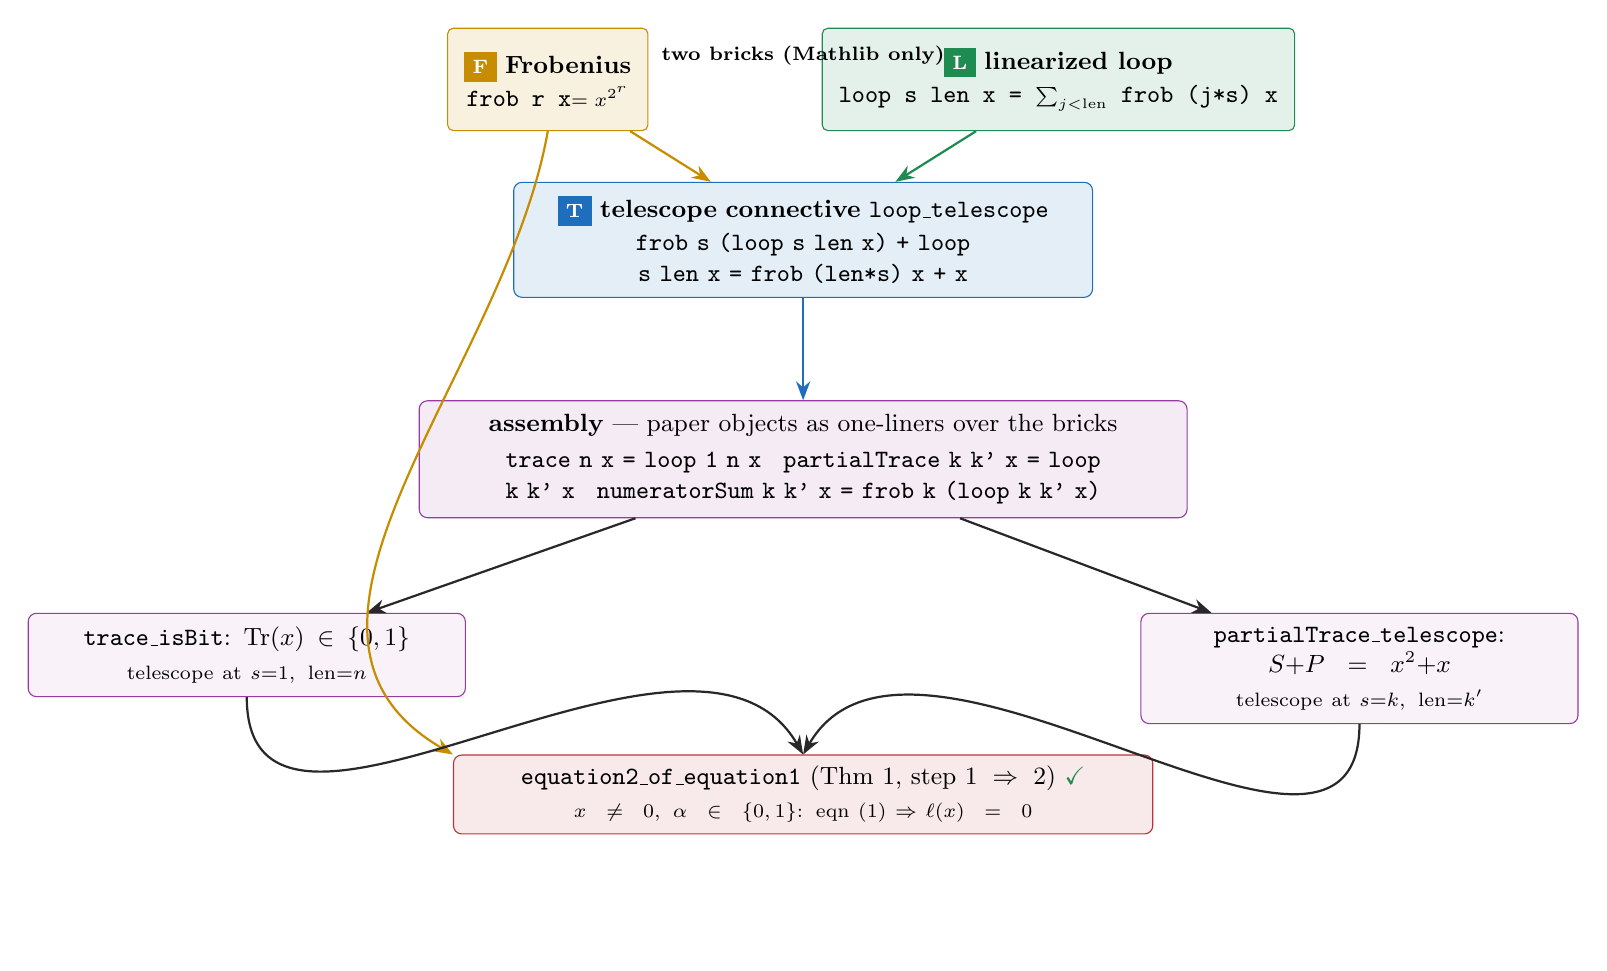
\begin{tikzpicture}[node distance=6mm]
% bricks
\node[brick,draw=faceF,fill=faceF!12] (F)
  {\bF\ \textbf{Frobenius}\\[1pt]\scriptsize\lc{frob r x}$=x^{2^r}$};
\node[brick,draw=faceL,fill=faceL!12,right=22mm of F] (L)
  {\bL\ \textbf{linearized loop}\\[1pt]\scriptsize\lc{loop s len x = }$\sum_{j<\text{len}}$\lc{ frob (j*s) x}};
\node[above=0.5mm of $(F)!0.5!(L)$,font=\scriptsize\bfseries] {two bricks (Mathlib only)};

% connective
\node[obj,draw=conn,fill=conn!12,below=13mm of $(F)!0.5!(L)$,text width=70mm] (T)
  {\bT\ \textbf{telescope connective} \lc{loop\_telescope}\\[1pt]
   \scriptsize\lc{frob s (loop s len x) + loop s len x = frob (len*s) x + x}};

% assembly (paper objects)
\node[obj,draw=asm,fill=asm!10,below=13mm of T,text width=94mm] (A)
  {\textbf{assembly} --- paper objects as one-liners over the bricks\\[2pt]
   \scriptsize
   \lc{trace n x = loop 1 n x}\quad
   \lc{partialTrace k k' x = loop k k' x}\quad
   \lc{numeratorSum k k' x = frob k (loop k k' x)}};

% two derived facts
\node[obj,draw=asm,fill=asm!6,below left=12mm and -6mm of A,text width=52mm] (bit)
  {\lc{trace\_isBit}: \(\mathrm{Tr}(x)\in\{0,1\}\)\\[1pt]
   \scriptsize telescope at \(s{=}1,\ \text{len}{=}n\)};
\node[obj,draw=asm,fill=asm!6,below right=12mm and -6mm of A,text width=52mm] (tel)
  {\lc{partialTrace\_telescope}: \(S{+}P=x^2{+}x\)\\[1pt]
   \scriptsize telescope at \(s{=}k,\ \text{len}{=}k'\)};

% headline
\node[thm,draw=res,fill=res!10,below=30mm of A,text width=86mm] (H)
  {\textbf{\lc{equation2\_of\_equation1}} (Thm 1, step $1\Rightarrow2$) \ck\\[1pt]
   \scriptsize \(x\neq0,\ \alpha\in\{0,1\}\): eqn (1) \(\Rightarrow\) \(\ell(x)=0\)};

% edges
\draw[dep,faceF] (F) -- (T);
\draw[dep,faceL] (L) -- (T);
\draw[dep,conn] (T) -- (A);
\draw[dep] (A) -- (bit);
\draw[dep] (A) -- (tel);
\draw[dep,faceF] (F.south) to[out=-100,in=150] (H.north west);
\draw[dep] (bit.south) to[out=-90,in=120] (H.north);
\draw[dep] (tel.south) to[out=-90,in=60] (H.north);
\end{tikzpicture}
\end{center}

\noindent The dependency edges are literal Lean \lc{import}s. The three objects
\lc{trace}, \lc{partialTrace}, \lc{numeratorSum} --- three separate definitions
in the earlier library --- are now a \emph{single} gadget \bL\ at different
settings, and the two telescoping proofs collapse to \emph{one} connective \bT.

%=====================================================================
\section{Brick \bF\ --- Frobenius (\texttt{DobbertinLego/Frobenius.lean})}

The doubling map on exponents, $x\mapsto x^{2^r}$. Its four laws are the entire
finite-field vocabulary the proof needs.
\begin{lean}
def frob (r : \(\mathbb{N}\)) (x : F) : F := x ^ (2 ^ r)
frob_add     : frob r (x + y) = frob r x + frob r y          \ck  -- additive
frob_comp    : frob a (frob b x) = frob (a + b) x            \ck  -- iterates compose
frob_periodic: |F|=2^n \(\Rightarrow\) frob r x = frob (r % n) x         \ck  -- period n
frob_card    : |F|=2^n \(\Rightarrow\) frob n x = x                     \ck  -- Fermat
\end{lean}

%=====================================================================
\section{Brick \bL\ + connective \bT\ (\texttt{DobbertinLego/Loop.lean})}

Gadget \bF\ \emph{closed into a loop} of length \lc{len} with step \lc{s}: the
running sum of the doubling map along an arithmetic progression of exponents.
\begin{center}
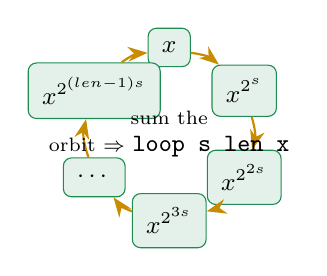
\begin{tikzpicture}[scale=1,every node/.style={font=\small}]
\def\R{1.1}
\foreach \a/\lab in {90/x,30/x^{2^{s}},-30/x^{2^{2s}},-90/x^{2^{3s}},
    -150/\cdots,150/x^{2^{(len-1)s}}}{
  \node[obj,draw=faceL,fill=faceL!12] (n\a) at (\a:\R) {$\lab$};}
\foreach \a/\b in {90/30,30/-30,-30/-90,-90/-150,-150/150,150/90}{
  \draw[arr,faceF] (n\a) to[bend left=16] (n\b);}
\node[align=center] at (0,0) {\scriptsize sum the\\[-1pt]\scriptsize orbit
  $\Rightarrow$ \lc{loop s len x}};
\end{tikzpicture}
\end{center}
\begin{lean}
def loop (s len : \(\mathbb{N}\)) (x : F) : F := \(\sum\)\_{j<len} frob (j*s) x
loop_succ     : loop s (len+1) x = loop s len x + frob (len*s) x       \ck
loop_telescope: frob s (loop s len x) + loop s len x
                  = frob (len*s) x + x                                 \ck  \bT
\end{lean}
\emph{The connective \bT.} One induction on \lc{len}: applying one more Frobenius
step (brick \bF, additive) to the loop and adding the loop back makes every
interior power appear twice, so it cancels in characteristic~2, leaving only the
two endpoints. This single lemma is the paper's ``add the $2^k$-th power of this
equation to itself''.

%=====================================================================
\section{Assembly (\texttt{DobbertinLego/Assembly.lean})}

The paper's objects are now one-liners; the two auxiliary facts are two uses of
\bT.
\begin{center}\small
\renewcommand{\arraystretch}{1.3}
\begin{tabular}{@{}l l l@{}}
\textbf{paper object} & \textbf{LEGO expression} & \textbf{Lean}\\ \hline
trace $\mathrm{Tr}(x)=\sum_{i<n}x^{2^i}$ & \bL\ at $s{=}1$ & \lc{trace n x = loop 1 n x}\\
partial trace $P(x)=\sum_{j<k'}x^{2^{jk}}$ & \bL\ at $s{=}k$ & \lc{partialTrace k k' x = loop k k' x}\\
numerator sum $S(x)=\sum_{i=1}^{k'}x^{2^{ik}}$ & \bF$\circ$\bL & \lc{numeratorSum k k' x = frob k (loop k k' x)}\\
\end{tabular}
\end{center}
\begin{lean}
numeratorSum_eq_frob_partialTrace : numeratorSum k k' x = partialTrace k k' x ^(2^k)  \ck  -- rfl
trace_isBit            : |F|=2^n \(\Rightarrow\) trace n x = 0 \(\vee\) trace n x = 1        \ck  -- \bT at s=1
partialTrace_telescope : |F|=2^n \(\to\) k*k'%n=1 \(\Rightarrow\)
                           numeratorSum k k' x + partialTrace k k' x = x^2 + x   \ck  -- \bT at s=k
\end{lean}
\emph{Two uses of one connective.} \lc{trace\_isBit} is \bT\ at $s{=}1,\ len{=}n$:
$\mathrm{Tr}^2+\mathrm{Tr}=\text{frob }n\,x+x=0$ (by \lc{frob\_card}), so
$\mathrm{Tr}$ is idempotent, hence a bit. \lc{partialTrace\_telescope} is \bT\ at
$s{=}k,\ len{=}k'$ with the endpoint $\text{frob }(k'k)\,x$ collapsed to $x^2$ by
\lc{frob\_periodic} and $k\cdot k'\equiv1\ (\mathrm{mod}\ n)$. And
$S=P^{2^k}$ holds \emph{by definition} (\lc{rfl}).

%=====================================================================
\section{The headline (\texttt{DobbertinLego.lean})}

\begin{center}
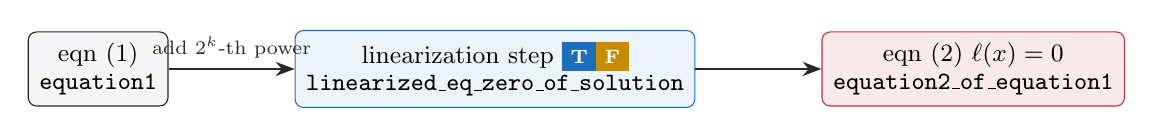
\begin{tikzpicture}[node distance=7mm and 16mm]
\node[thm,fill=soft] (e1) {eqn (1)\\[-1pt]\scriptsize\lc{equation1}};
\node[thm,right=of e1,draw=conn,fill=conn!8] (lin)
  {linearization step \bT\bF\\[-1pt]\scriptsize\lc{linearized\_eq\_zero\_of\_solution}};
\node[thm,right=of lin,draw=res,fill=res!10] (e2)
  {eqn (2) \(\ell(x)=0\)\\[-1pt]\scriptsize\lc{equation2\_of\_equation1}};
\draw[dep] (e1) -- node[above,font=\scriptsize]{add $2^k$-th power} (lin);
\draw[dep] (lin) -- (e2);
\end{tikzpicture}
\end{center}
\begin{lean}
def equation1 (n k k' \(\alpha\) : \(\mathbb{N}\)) (c x : F) : Prop :=
  c * x^(2^k+1) = numeratorSum k k' x + (\(\alpha\):F) * trace n x
def linearized (k : \(\mathbb{N}\)) (c x : F) : F :=
  c^(2^k) * x^(2^(2*k)) + x^(2^k) + c*x + 1

theorem equation2_of_equation1 (hn : |F| = 2^n) (hkk' : k*k' % n = 1)
    (h\(\alpha\) : \(\alpha\)=0 \(\vee\) \(\alpha\)=1) (hx : x \(\neq\) 0) (h : equation1 n k k' \(\alpha\) c x) :
    linearized k c x = 0                                                  \ck
\end{lean}
The proof: collapse $\alpha\cdot\mathrm{Tr}(x)$ to a bit $\varepsilon$ (via
\lc{trace\_isBit}); solve (1) for $P$ using $S=P^{2^k}$ and the telescope
$S+P=x^2+x$; raise to the $2^k$ power (brick \bF\ additive, $\varepsilon^{2^k}=
\varepsilon$); cancel $\varepsilon$ and divide by $x^{2^k}\neq0$ to read off
$\ell(x)=0$.
\emph{Why $x\neq0$.} At $x=0$ the cleared (1) holds vacuously ($0=0$) while
$\ell(0)=1\neq0$; the hypothesis is genuinely required.

%=====================================================================
\section*{Compositional build diagram}

\begin{center}
\begin{tikzcd}[column sep=large,row sep=large]
\text{\bF\ \lc{frob}} \arrow[r,"\text{additive}"] \arrow[dr,"\text{compose}"']
  & \text{\bL\ \lc{loop}} \arrow[d,"\text{induction}"] \\
& \text{\bT\ \lc{loop\_telescope}}
  \arrow[r,"s=1"] \arrow[d,"s=k"']
  & \text{\lc{trace\_isBit}} \arrow[d] \\
& \text{\lc{partialTrace\_telescope}} \arrow[r]
  & \text{\lc{linearized\_eq\_zero\_of\_solution}} \arrow[d] \\
&& \text{\lc{equation2\_of\_equation1}}
\end{tikzcd}
\end{center}

\begin{note}
\textbf{One sentence.} The step $(1)\Rightarrow(2)$ of Dobbertin's Theorem~1 is
\emph{one} gadget --- the linearized Frobenius loop \bL\ built on the doubling
brick \bF\ --- together with its \emph{one} telescoping connective \bT; the
paper's trace, partial trace and numerator sum are that gadget at three settings,
its ``add the $2^k$-th power'' move is that connective, and the headline is a
short assembly on top. \emph{Scope:} this covers the first step only; the two
root-counting cases, Theorem~1 proper and the difference-set half are not part of
this minimal library.
\end{note}

\vfill
\begin{center}\scriptsize
Source: \lc{DobbertinLego/} (\lc{Frobenius}, \lc{Loop}, \lc{Assembly}) and
\lc{DobbertinLego.lean}. Paper: H.~Dobbertin, \emph{Kasami Power Functions,
Permutation Polynomials and Cyclic Difference Sets} (1999), proof of Theorem~1,
step (1)\,$\Rightarrow$\,(2).
\end{center}

\end{document}
